\documentclass[aspectratio=169,xcolor={table,dvipsnames}]{beamer}

\usetheme{default}

% ---------- Core Packages ----------
\usepackage[utf8]{inputenc}
\usepackage{booktabs}
\usepackage{tabularx}
\usepackage{array}
\usepackage{amsmath}
\usepackage{amssymb}
\usepackage{tikz}
\usepackage{graphicx}
\usepackage{colortbl}
\usepackage{ragged2e}
\usepackage{tcolorbox}

\usetikzlibrary{positioning,trees,shapes,arrows.meta,calc}
\usepackage{multimedia}

% ============================================================
% PRESENTATION COLOR PALETTE (Amrita Theme)
% ============================================================

\definecolor{maroon}{RGB}{165,0,52}
\definecolor{amritaMaroon}{RGB}{165,0,52}
\definecolor{deepmaroon}{RGB}{145,0,45}
\definecolor{royalblue}{RGB}{0,55,190}

\definecolor{lightblue}{RGB}{236,246,253}
\definecolor{lightgreen}{RGB}{236,250,240}
\definecolor{lightyellow}{RGB}{255,250,232}
\definecolor{lightpink}{RGB}{254,241,245}
\definecolor{lightcyan}{RGB}{235,250,250}
\definecolor{lightorange}{RGB}{255,246,236}
\definecolor{lightpurple}{RGB}{246,242,254}

\definecolor{darktext}{RGB}{35,35,35}
\definecolor{darkred}{RGB}{180,0,0}

% ============================================================
% GLOBAL BEAMER STYLING
% ============================================================

\setbeamercolor{normal text}{fg=darktext,bg=white}
\setbeamercolor{structure}{fg=maroon}

\setbeamercolor{frametitle}{fg=white,bg=maroon}
\setbeamerfont{frametitle}{size=\large,series=\bfseries}

\setbeamercolor{title}{fg=maroon}
\setbeamercolor{subtitle}{fg=darktext}
\setbeamercolor{author}{fg=darktext}
\setbeamercolor{institute}{fg=darktext}

\setbeamercolor{block title}{fg=white,bg=maroon}
\setbeamercolor{block body}{fg=darktext,bg=lightpink}

\setbeamercolor{alerted text}{fg=maroon}

\setbeamercolor{itemize item}{fg=maroon}
\setbeamercolor{itemize subitem}{fg=maroon}

\setbeamertemplate{navigation symbols}{}

% ============================================================
% FOOTLINE
% ============================================================

\setbeamertemplate{footline}{%
    \leavevmode%
    \hbox{%
        \begin{beamercolorbox}[wd=\paperwidth,ht=0.08cm,dp=0cm]{frametitle}%
        \end{beamercolorbox}%
    }%
}

% ============================================================
% CLEAN HEADER BAR
% ============================================================

\setbeamertemplate{frametitle}{%
    \nointerlineskip%
    \begin{beamercolorbox}[wd=\paperwidth,leftskip=0.5cm,rightskip=0.5cm,vmode]{frametitle}%
        \vskip 0.20cm%
        {\usebeamerfont{frametitle}\insertframetitle\strut\par}%
        \vskip 0.20cm%
    \end{beamercolorbox}%
}

% ============================================================
% HELPER COMMANDS
% ============================================================

\newcommand{\blue}[1]{\textcolor{royalblue}{\textbf{#1}}}
\newcommand{\maroonText}[1]{\textcolor{maroon}{\textbf{#1}}}

\title{\textcolor{maroon}{\textbf{CFG Grammar Compiler --- Extracted Slides (V3)}}}
\subtitle{Sign Language to 3D Avatar Generation}
\date{}

% ============================================================
% DOCUMENT
% ============================================================
\begin{document}

\begin{frame}[plain]
\titlepage
\end{frame}

% ============================================================
% SLIDE 12: FORMAL 4-TUPLE GRAMMAR SPECIFICATION
% ============================================================
\section{CFG Grammar Compiler}
\begin{frame}[t]{12. Context-Free Grammar: Formal 4-Tuple Specification}
\vspace{-0.1cm}
\begin{center}
    \scriptsize\textit{\textcolor{amritaMaroon}{Formal theoretical definition $G = (V, T, P, S)$ and project mapping (Hopcroft et al., 2006)}}
\end{center}

\vspace{-1.5mm}
\setbeamercolor{block title}{fg=white,bg=maroon}
\setbeamercolor{block body}{fg=darktext,bg=lightpink}
\begin{block}{Theoretical Role: Lexer vs. Parser Architecture}
    \fontsize{6.8pt}{8.6pt}\selectfont
    The feature extraction pipeline (BiGRU / 10 heuristic modules) acts as the \textbf{Lexer} (producing unconstrained phonetic probabilities). The CFG compiler acts as the \textbf{Parser} (enforcing strict phonological syntax), converting chaotic predictions into a deterministic HamNoSys sequence for 3D avatar execution.
\end{block}

\vspace{1.2mm}
\centering
\setlength{\tabcolsep}{4pt}
\renewcommand{\arraystretch}{1.22}
{\fontsize{6.8pt}{8.6pt}\selectfont
\begin{tabular}{|>{\centering\arraybackslash\bfseries}p{0.8cm}|>{\raggedright\arraybackslash\bfseries}p{2.3cm}|>{\raggedright\arraybackslash}p{6.4cm}|>{\raggedright\arraybackslash}p{3.0cm}|}
    \hline
    \rowcolor{maroon}
    \textcolor{white}{\textbf{Tuple}} & 
    \textcolor{white}{\textbf{Grammar Component}} & 
    \textcolor{white}{\textbf{Formal Mathematical Definition \& Disjoint Alphabet}} & 
    \textcolor{white}{\textbf{Role in SignBridge V2}} \\
    \hline
    \rowcolor{lightblue} 
    $V$ & Variables / Non-Terminals ($|V|=17$) & 
    $V = \{\langle\text{Sign}\rangle, \langle\text{ManualConfig}\rangle, \langle\text{Symmetry}\rangle, \langle\text{SingleHand}\rangle, \langle\text{DualHand}\rangle, \langle\text{Orientation}\rangle, \langle\text{Handshape}\rangle, \dots\}$ & 
    Syntactic categories mapping to Stokoe's Tab-Dez-Sig phonological constituents. \\
    \hline
    \rowcolor{lightgreen} 
    $T$ & Terminals / Alphabet ($|T|=83$) & 
    \textbf{Disjoint Partition Alphabet:}\\[0.5mm]
    $\mathbf{T = \bigsqcup_{k=1}^8 T_k = T_{\text{symm}} \sqcup T_{\text{hs}} \sqcup T_{\text{ext}} \sqcup T_{\text{palm}} \sqcup T_{\text{loc}} \sqcup T_{\text{cont}} \sqcup T_{\text{mov}} \sqcup T_{\text{trans}}}$\\[0.5mm]
    $\bullet\; T_{\text{symm}} (3):\; \{\texttt{hamsymmlr}, \texttt{hamnonipsi}, \texttt{hamplus}\}$\\[0.2mm]
    $\bullet\; T_{\text{hs}} (20):\; \text{Handshapes } \{\texttt{hamflathand}, \texttt{hamfist}, \dots\}$\\[0.2mm]
    $\bullet\; T_{\text{ext}} (10):\; \text{Extended fingers } \{\texttt{hamextfingeru}, \dots\}$\\[0.2mm]
    $\bullet\; T_{\text{palm}} (8):\; \text{Palm facings } \{\texttt{hampalmu}, \texttt{hampalmd}, \dots\}$\\[0.2mm]
    $\bullet\; T_{\text{loc}} (25):\; \text{Body locations } \{\texttt{hamchest}, \texttt{hamhead}, \dots\}$\\[0.2mm]
    $\bullet\; T_{\text{cont}} (4):\; \text{Contact types } \{\texttt{hamtouch}, \texttt{hamclose}, \dots\}$\\[0.2mm]
    $\bullet\; T_{\text{mov}} (12):\; \text{Movements } \{\texttt{hammoveo}, \texttt{hamcircle}, \dots\}$\\[0.2mm]
    $\bullet\; T_{\text{trans}} (1):\; \text{Dynamic posture replace } \{\texttt{hamreplace}\}$ & 
    83 atomic HamNoSys phonetic tokens driving WebGL avatar bone rotations. \\
    \hline
    \rowcolor{lightyellow} 
    $P$ & Production Rules ($|P|=17$) & 
    Rewriting rules in Backus-Naur Form (BNF): $A \to \alpha$, where $A \in V$ and $\alpha \in (V \cup T)^*$ & 
    Enforces linear syntax order: $\text{Hand} \to \text{Loc} \to \text{Contact} \to \text{Movement}$. \\
    \hline
    \rowcolor{lightorange} 
    $S$ & Start Symbol & 
    $S = \langle\text{Sign}\rangle \in V$ & 
    Root sentence symbol representing the complete gesture derivation. \\
    \hline
\end{tabular}
}

\vspace{1.2mm}
\fcolorbox{amritaMaroon}{white}{
    \parbox{0.96\textwidth}{
        \centering\fontsize{6.4pt}{8.0pt}\selectfont
        \textbf{Formal Language Guarantee:} The generated sign language $L(G) = \{w \in T^* \mid S \implies^* w\}$ is guaranteed to be context-free and parseable by the CWASA WebGL SiGML engine without runtime ambiguity.
    }
}
\end{frame}

% ============================================================
% SLIDE 12a-1: FORMAL CFG PRODUCTION RULES (CORE BACKBONE)
% ============================================================
\begin{frame}[t]{12a. Formal CFG Production Rules: Core Structural Backbone}
\vspace{-0.1cm}
\begin{center}
    \scriptsize\textit{\textcolor{amritaMaroon}{Linguistically grounded rewrite rules enforcing strict phonological ordering (Rules P1--P5)}}
\end{center}

\vspace{-1.5mm}
\centering
\setlength{\tabcolsep}{4pt}
\renewcommand{\arraystretch}{1.28}
{\fontsize{7.2pt}{9.2pt}\selectfont
\begin{tabular}{|>{\centering\arraybackslash\bfseries}p{1.0cm}|>{\raggedright\arraybackslash\bfseries}p{2.6cm}|>{\raggedright\arraybackslash}p{5.8cm}|>{\raggedright\arraybackslash}p{3.2cm}|}
    \hline
    \rowcolor{maroon}
    \textcolor{white}{\textbf{Rule ID}} & 
    \textcolor{white}{\textbf{Constituent Name}} & 
    \textcolor{white}{\textbf{Production Rule in Backus-Naur Form (BNF)}} & 
    \textcolor{white}{\textbf{Linguistic Meaning \& Scope}} \\
    \hline
    \rowcolor{lightblue} 
    \textbf{P1} & Root Sign & 
    $\langle\text{Sign}\rangle \to \langle\text{ManualConfig}\rangle \;\mid\; \langle\text{Symmetry}\rangle \;\langle\text{ManualConfig}\rangle$ & 
    Top-level sentence expansion with optional bilateral symmetry prefix. \\
    \hline
    \rowcolor{lightgreen} 
    \textbf{P2} & Manual Configuration & 
    $\langle\text{ManualConfig}\rangle \to \langle\text{SingleHand}\rangle \;\langle\text{Location}\rangle \;[\langle\text{Contact}\rangle] \;[\langle\text{Movement}\rangle] \;[\langle\text{StateTransition}\rangle]$ & 
    Core linear sign syntagm: Hand posture followed by body anchor and optional modifiers. \\
    \hline
    \rowcolor{lightyellow} 
    \textbf{P3} & Single-Hand Form & 
    $\langle\text{SingleHand}\rangle \to \langle\text{Handshape}\rangle \;\langle\text{Orientation}\rangle$ & 
    Phonological hand unit combining anatomical handshape and 3D spatial attitude. \\
    \hline
    \rowcolor{lightcyan} 
    \textbf{P4} & Dual-Hand Structure & 
    $\langle\text{DualHand}\rangle \to \langle\text{SingleHand}\rangle \;\texttt{hamplus}\; \langle\text{SingleHand}\rangle$ & 
    Asymmetric two-handed sign where dominant hand acts on secondary base hand. \\
    \hline
    \rowcolor{lightorange} 
    \textbf{P5} & 3D Spatial Orientation & 
    $\langle\text{Orientation}\rangle \to \langle\text{ExtFinger}\rangle \;\langle\text{PalmOri}\rangle$ & 
    Orthogonal coordinate pair: extended finger vector $\vec{f}$ and palm normal vector $\vec{n}$. \\
    \hline
\end{tabular}
}

\vspace{2.5mm}
\fcolorbox{amritaMaroon}{lightyellow}{
    \parbox{0.96\textwidth}{
        \fontsize{6.6pt}{8.4pt}\selectfont
        \textbf{Grammar Conventions \& BNF Operators:}
        \begin{itemize}\setlength{\itemsep}{0.04cm}
            \item $\to$ : Rewriting operator (expands non-terminal on left into constituent string on right).
            \item $\mid$ : Syntactic alternation (disjunctive choice between valid structures).
            \item $[\cdot]$ : Optional constituent (instantiated during derivation only when physical feature is detected).
            \item Maps directly to Stokoe's Sign Architecture: \textbf{Tab} (Location: P2), \textbf{Dez} (Handshape: P3), \textbf{Sig} (Orientation \& Movement: P5, P2).
        \end{itemize}
    }
}
\end{frame}

% ============================================================
% SLIDE 12a-2: FORMAL CFG PRODUCTION RULES (MODIFIERS & GUARDS)
% ============================================================
\begin{frame}[t]{12a-2. Formal CFG Production Rules: Modifiers, Transitions \& Semantic Guards}
\vspace{-0.1cm}
\begin{center}
    \scriptsize\textit{\textcolor{amritaMaroon}{Dynamic posture transitions (P6--P17) and real-time biomechanical constraint enforcement}}
\end{center}

\vspace{-1.5mm}
\centering
\setlength{\tabcolsep}{4pt}
\renewcommand{\arraystretch}{1.22}
{\fontsize{6.8pt}{8.6pt}\selectfont
\begin{tabular}{|>{\centering\arraybackslash\bfseries}p{1.1cm}|>{\raggedright\arraybackslash\bfseries}p{2.5cm}|>{\raggedright\arraybackslash}p{5.8cm}|>{\raggedright\arraybackslash}p{3.2cm}|}
    \hline
    \rowcolor{maroon}
    \textcolor{white}{\textbf{Rule ID}} & 
    \textcolor{white}{\textbf{Constituent}} & 
    \textcolor{white}{\textbf{Production Rule in BNF Form}} & 
    \textcolor{white}{\textbf{Linguistic Meaning}} \\
    \hline
    \rowcolor{lightpink} 
    \textbf{P6--P8} & Optional Modifiers & 
    $\langle\text{OptContact}\rangle \to \langle\text{Contact}\rangle \mid \varepsilon \quad \langle\text{OptMov}\rangle \to \langle\text{Mov}\rangle \mid \varepsilon$ & 
    $\varepsilon$-productions allowing clean reduction when contact or movement is absent. \\
    \hline
    \rowcolor{lightpurple} 
    \textbf{P9} & State Transition & 
    $\langle\text{StateTransition}\rangle \to \texttt{hamreplace} \;\langle\text{Handshape}\rangle \;\langle\text{Orientation}\rangle \;[\langle\text{Location}\rangle]$ & 
    Mid-sign dynamic posture switch (e.g. open-to-close handshape or wrist turn). \\
    \hline
    \rowcolor{lightblue} 
    \textbf{P11} & Symmetry Operators & 
    $\langle\text{Symmetry}\rangle \to \texttt{hamsymmlr} \mid \texttt{hamnonipsi}$ & 
    Mirror bilateral symmetry vs non-ipsilateral signing hand configuration. \\
    \hline
    \rowcolor{white} 
    \textbf{P12--P17} & Terminal Leaves & 
    $\langle\text{HS}\rangle \to \texttt{hamflathand} \mid \dots \quad \langle\text{Loc}\rangle \to \texttt{hamchest} \mid \dots$ & 
    Grounding to 83 atomic HamNoSys phonetic tokens in alphabet $T$. \\
    \hline
\end{tabular}
}

\vspace{1.5mm}
\begin{columns}[T]
    \column{0.49\textwidth}
    \setbeamercolor{block title}{fg=white,bg=maroon}
    \setbeamercolor{block body}{fg=darktext,bg=lightgreen}
    \begin{block}{Grammatical Semantic Constraints}
        \fontsize{6.6pt}{8.4pt}\selectfont
        $\bullet$ \textbf{Contact Proximity Gating:} Contact tokens (\texttt{hamtouch}) are valid \textbf{only} when hand is near body surfaces (chest, lips, chin). Floating contact in empty neutral space is rejected.\\
        $\bullet$ \textbf{Monotonic Ordering:} Enforces rigid token sequence, rejecting disordered asynchronous arrivals.
    \end{block}

    \column{0.49\textwidth}
    \setbeamercolor{block title}{fg=white,bg=maroon}
    \setbeamercolor{block body}{fg=darktext,bg=lightyellow}
    \begin{block}{Inverse Kinematics (IK) Sanitization}
        \fontsize{6.6pt}{8.4pt}\selectfont
        $\bullet$ Overrides anatomically impossible joint combinations before WebGL avatar rendering.\\
        $\bullet$ \textbf{Concrete Rule:} If $\text{Location} = \texttt{hamchest}$ and $\text{ExtFinger} = \texttt{hamextfingerd}$ (downward pointing fingers at chest), sanitize to \texttt{hamextfingerl} to prevent unphysical $180^\circ$ wrist dislocation.
    \end{block}
\end{columns}
\end{frame}

% ============================================================
% SLIDE 12b: PIPELINE TRACE (BOXED GRAPH)
% ============================================================
\begin{frame}[t]{12b. End-to-End Pipeline Tracing: From Video to HamNoSys String}
\vspace{-0.1cm}
\begin{center}
    \scriptsize\textit{\textcolor{amritaMaroon}{Systematic transformation of 150-frame video inputs into deterministic HamNoSys syntax}}
\end{center}

\vspace{-1.5mm}
\centering
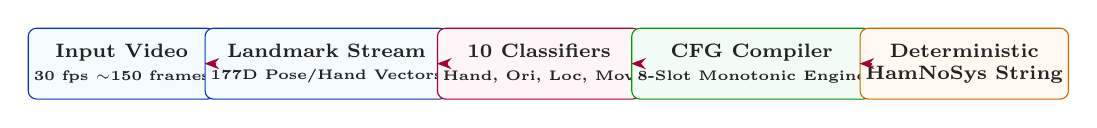
\begin{tikzpicture}[
    node distance=0.35cm,
    ibox/.style={rectangle, draw=royalblue, fill=lightblue!60, text=darktext, font=\bfseries\fontsize{6.6pt}{8.0pt}\selectfont, align=center, rounded corners=3pt, minimum height=0.9cm, minimum width=2.2cm, inner sep=2pt},
    pbox/.style={rectangle, draw=amritaMaroon, fill=lightpink!70, text=darktext, font=\bfseries\fontsize{6.6pt}{8.0pt}\selectfont, align=center, rounded corners=3pt, minimum height=0.9cm, minimum width=2.4cm, inner sep=2pt},
    cbox/.style={rectangle, draw=green!60!black, fill=lightgreen!70, text=darktext, font=\bfseries\fontsize{6.6pt}{8.0pt}\selectfont, align=center, rounded corners=3pt, minimum height=0.9cm, minimum width=2.3cm, inner sep=2pt},
    obox/.style={rectangle, draw=orange!80!black, fill=lightorange!70, text=darktext, font=\bfseries\fontsize{6.6pt}{8.0pt}\selectfont, align=center, rounded corners=3pt, minimum height=0.9cm, minimum width=2.4cm, inner sep=2pt},
    flowarr/.style={-{Stealth[scale=0.8]}, thick, amritaMaroon}
]
    \node (v1) at (0,0) [ibox] {Input Video\\{\tiny 30 fps $\sim$150 frames}};
    \node (v2) at (2.6,0) [ibox] {Landmark Stream\\{\tiny 177D Pose/Hand Vectors}};
    \node (v3) at (5.3,0) [pbox] {10 Classifiers\\{\tiny Hand, Ori, Loc, Mov}};
    \node (v4) at (8.0,0) [cbox] {CFG Compiler\\{\tiny 8-Slot Monotonic Engine}};
    \node (v5) at (10.7,0) [obox] {Deterministic\\HamNoSys String};

    \draw [flowarr] (v1) -- (v2);
    \draw [flowarr] (v2) -- (v3);
    \draw [flowarr] (v3) -- (v4);
    \draw [flowarr] (v4) -- (v5);
\end{tikzpicture}

\vspace{2.0mm}
\begin{columns}[T]
    \column{0.49\textwidth}
    \setbeamercolor{block title}{fg=white,bg=maroon}
    \setbeamercolor{block body}{fg=darktext,bg=lightblue}
    \begin{block}{Multi-Stream Input Signal Processing}
        \fontsize{6.8pt}{8.6pt}\selectfont
        \begin{enumerate}\setlength{\itemsep}{0.06cm}
            \item \textbf{Video Decode:} OpenCV decodes raw camera frames (30 fps).
            \item \textbf{Kinematic Extraction:} Single-pass MediaPipe extracts 177 normalized coordinates per frame (wrist, 21 hand $\times 2$, 17 pose).
            \item \textbf{Parallel Classification:} 10 heuristic modules run concurrently:
            \begin{itemize}\setlength{\itemsep}{0.02cm}
                \item Handshape $\to$ Finger joint curl dot products
                \item Orientation $\to$ 3D vector normal $\vec{u} \times \vec{v}$
                \item Upper Body \& Face $\to$ Body-scale ratio $\frac{\text{dist}}{S_w} < 0.25$
                \item Movement \& Contact $\to$ Multi-frame trajectories
            \end{itemize}
        \end{enumerate}
    \end{block}

    \column{0.49\textwidth}
    \setbeamercolor{block title}{fg=white,bg=maroon}
    \setbeamercolor{block body}{fg=darktext,bg=lightgreen}
    \begin{block}{Deterministic Syntactic Reduction}
        \fontsize{6.8pt}{8.6pt}\selectfont
        \begin{enumerate}\setlength{\itemsep}{0.06cm}
            \item \textbf{Input to Parser:} Receives 10 raw, asynchronous prediction arrays (each containing $\sim$150 frame-level labels).
            \item \textbf{Syntactic Compilation:} The CFG compiler filters transient noise, resolves modal consensus, and applies leftmost BNF derivations.
            \item \textbf{Canonical Output:} Emits a minimal, non-redundant string (5--7 tokens) strictly conforming to Chomsky hierarchy.
            \item \textbf{Avatar Driving:} SiGML synthesis engine maps tokens to XML $\to$ real-time WebGL CWASA 3D avatar animation.
        \end{enumerate}
    \end{block}
\end{columns}
\end{frame}

% ============================================================
% SLIDE 12b-2: 5-STAGE PHONETIC FILTRATION & STABILIZATION
% ============================================================
\begin{frame}[t]{12b-2. 5-Stage Real-Time Phonetic Filtration \& Sequence Normalization Engine}
\vspace{-0.1cm}
\begin{center}
    \scriptsize\textit{\textcolor{amritaMaroon}{Multi-tier noise rejection preventing token jumbling, hallucinations, and avatar crashes}}
\end{center}

\vspace{-1.5mm}
\begin{columns}[T]
    \column{0.49\textwidth}
    \setbeamercolor{block title}{fg=white,bg=maroon}
    \setbeamercolor{block body}{fg=darktext,bg=lightyellow}
    \begin{block}{Stage 1: Temporal Phase Segmentation}
        \fontsize{6.6pt}{8.4pt}\selectfont
        $\bullet$ Discards frames 0--14\% (hand-raising onset noise) and 50--54\% (inter-stroke transitions).\\
        $\bullet$ Isolates \textbf{Phase 1} (15--50\%) and \textbf{Phase 2} (55--100\%) for pristine sign execution.
    \end{block}

    \setbeamercolor{block title}{fg=white,bg=maroon}
    \setbeamercolor{block body}{fg=darktext,bg=lightblue}
    \begin{block}{Stage 2: Statistical Modal Consensus Voting}
        \fontsize{6.6pt}{8.4pt}\selectfont
        $\bullet$ Evaluates $\text{Counter}(\text{phase}).\text{most\_common}(1)$ across active windows.\\
        $\bullet$ Eliminates transient 2-frame tracking glitches (e.g. 142 \texttt{hamflathand} vs 3 \texttt{hamfist} $\to$ only \texttt{hamflathand} survives).
    \end{block}

    \setbeamercolor{block title}{fg=white,bg=maroon}
    \setbeamercolor{block body}{fg=darktext,bg=lightgreen}
    \begin{block}{Stage 3: Lexical Whitelist Validation}
        \fontsize{6.6pt}{8.4pt}\selectfont
        $\bullet$ Validates every candidate token against the canonical alphabet $T$ ($|T|=83$).\\
        $\bullet$ Instantly purges out-of-vocabulary artifacts and undefined strings.
    \end{block}

    \column{0.49\textwidth}
    \setbeamercolor{block title}{fg=white,bg=maroon}
    \setbeamercolor{block body}{fg=darktext,bg=lightorange}
    \begin{block}{Stage 4: Biomechanical \& IK Sanitization}
        \fontsize{6.6pt}{8.4pt}\selectfont
        $\bullet$ Intercepts impossible joint angles (e.g. downward-facing palm while hand is touching forehead).\\
        $\bullet$ Sanitizes to nearest physically valid anatomical configuration before avatar XML synthesis.
    \end{block}

    \setbeamercolor{block title}{fg=white,bg=maroon}
    \setbeamercolor{block body}{fg=darktext,bg=lightpink}
    \begin{block}{Stage 5: Monotonic Chomsky Structural Assembly}
        \fontsize{6.6pt}{8.4pt}\selectfont
        $\bullet$ Tokens are placed into predefined structural slots:
        $$\mathbf{\text{Symmetry} \to \text{Handshape} \to \text{Orientation} \to \text{Location} \to [\text{Contact}] \to [\text{Movement}]}$$
        $\bullet$ \textbf{Order Invariance:} Output order is governed strictly by linguistic production rules (P1--P17), \textbf{never} by frame detection arrival time!
    \end{block}
\end{columns}
\end{frame}

% ============================================================
% SLIDE 12c: LEFTMOST CFG GRAMMAR DERIVATION
% ============================================================
\begin{frame}[t]{12c. Leftmost CFG Grammar Derivation: Symmetric Sign ``BOOK''}
\vspace{-0.1cm}
\begin{center}
    \scriptsize\textit{\textcolor{amritaMaroon}{Step-by-step mathematical derivation from consensus module inputs to accepted terminal string}}
\end{center}

\vspace{-1.5mm}
\fcolorbox{amritaMaroon}{lightblue!40}{
    \parbox{0.96\textwidth}{
        \fontsize{6.6pt}{8.4pt}\selectfont
        \textbf{Consensus Module Inputs (Sign ``BOOK'', 150 Frames):} \quad
        $\texttt{Handshape} = \texttt{hamflathand}\; (97.9\%), \quad \texttt{Orientation} = (\texttt{hamextfingeru}, \texttt{hampalmu}), \quad \texttt{Location} = \texttt{hamchest}, \quad \texttt{Contact} = \texttt{hamtouch}, \quad \texttt{Movement} = \texttt{hammoveo}, \quad \texttt{Symmetry} = \texttt{hamsymmlr}$
    }
}

\vspace{2.0mm}
\setbeamercolor{block title}{fg=white,bg=maroon}
\setbeamercolor{block body}{fg=darktext,bg=lightpink!50}
\begin{block}{Formal Leftmost Grammar Derivation Sequence: $S \implies^* w \in T^*$}
    \fontsize{6.8pt}{9.0pt}\selectfont
    \begin{align*}
        \langle\text{Sign}\rangle 
        &\implies \langle\text{Symmetry}\rangle \;\langle\text{ManualConfig}\rangle && [\text{Rule P1: Root Sign Expansion}] \\
        &\implies \texttt{hamsymmlr} \;\langle\text{ManualConfig}\rangle && [\text{Rule P11: Bilateral Symmetry Leaf}] \\
        &\implies \texttt{hamsymmlr} \;\langle\text{SingleHand}\rangle \;\langle\text{Location}\rangle \;\langle\text{OptContact}\rangle \;\langle\text{OptMovement}\rangle \;\langle\text{OptTrans}\rangle && [\text{Rule P2: Core Syntagm Expansion}] \\
        &\implies \texttt{hamsymmlr} \;\langle\text{Handshape}\rangle \;\langle\text{Orientation}\rangle \;\langle\text{Location}\rangle \;\langle\text{OptContact}\rangle \;\dots && [\text{Rule P3: Single-Hand Structure}] \\
        &\implies \texttt{hamsymmlr hamflathand} \;\langle\text{Orientation}\rangle \;\langle\text{Location}\rangle \;\langle\text{OptContact}\rangle \;\dots && [\text{Rule P12: Handshape Terminal Leaf}] \\
        &\implies \texttt{hamsymmlr hamflathand hamextfingeru hampalmu} \;\langle\text{Location}\rangle \;\dots && [\text{Rules P5, P13, P14: 3D Orientation Leaves}] \\
        &\implies \texttt{hamsymmlr hamflathand hamextfingeru hampalmu hamchest} \;\langle\text{OptContact}\rangle \;\dots && [\text{Rule P15: Body Location Terminal Leaf}] \\
        &\implies \dots \;\texttt{hamchest hamtouch} \;\langle\text{OptMovement}\rangle \;\langle\text{OptTransition}\rangle && [\text{Rules P6, P16: Physical Contact Leaf}] \\
        &\implies \dots \;\texttt{hamtouch hammoveo} \;\langle\text{OptTransition}\rangle && [\text{Rules P7, P17: Motion Vector Leaf}] \\
        &\implies^* \mathbf{\texttt{hamsymmlr hamflathand hamextfingeru hampalmu hamchest hamtouch hammoveo}} && [\text{Rule P8: } \langle\text{OptTrans}\rangle \to \varepsilon]
    \end{align*}
\end{block}

\vspace{1.0mm}
\centering
\fcolorbox{green!60!black}{lightgreen}{
    \parbox{0.96\textwidth}{
        \centering\fontsize{6.8pt}{8.6pt}\selectfont
        \textbf{Ground Truth Dictionary Verification:} \textbf{7 / 7 Tokens Match Perfectly (100.0\% Precision, Zero Grammar Violations)}
    }
}
\end{frame}

% ============================================================
% SLIDE 12d-1: AUTOMATED BENCHMARK VERIFICATION (TIKZ FLOW)
% ============================================================
\begin{frame}[t]{12d. Automated Benchmark Verification: 170-Gloss Ground Truth}
\vspace{-0.1cm}
\begin{center}
    \scriptsize\textit{\textcolor{amritaMaroon}{Automated end-to-end evaluation against our curated 170-gloss linguistic dictionary}}
\end{center}

\vspace{-1.5mm}
\centering

\begin{tikzpicture}[
    node distance=0.4cm,
    gbox/.style={rectangle, draw=amritaMaroon, fill=lightpink!80, text=darktext, font=\bfseries\fontsize{6.6pt}{8.0pt}\selectfont, align=center, rounded corners=3pt, minimum height=0.95cm, minimum width=2.5cm, inner sep=2pt},
    tbox/.style={rectangle, draw=royalblue, fill=lightblue!70, text=darktext, font=\bfseries\fontsize{6.6pt}{8.0pt}\selectfont, align=center, rounded corners=3pt, minimum height=0.95cm, minimum width=2.5cm, inner sep=2pt},
    kbox/.style={rectangle, draw=green!60!black, fill=lightgreen!70, text=darktext, font=\bfseries\fontsize{6.6pt}{8.0pt}\selectfont, align=center, rounded corners=3pt, minimum height=0.95cm, minimum width=2.5cm, inner sep=2pt},
    obox/.style={rectangle, draw=orange!80!black, fill=lightorange!70, text=darktext, font=\bfseries\fontsize{6.6pt}{8.0pt}\selectfont, align=center, rounded corners=3pt, minimum height=0.95cm, minimum width=2.5cm, inner sep=2pt},
    flowarr/.style={-{Stealth[scale=0.85]}, thick, amritaMaroon}
]
    \node (n1) at (0,0) [gbox] {170 Curated ISL Signs\\{\tiny Curated JSON Corpus}};
    \node (n2) at (3.0,0) [tbox] {7 Phonetic Features\\{\tiny HS, Ext, Palm, Loc, Mov\dots}};
    \node (n3) at (6.0,0) [tbox] {CFG Compiler\\{\tiny Whitelist + BNF Rules}};
    \node (n4) at (9.0,0) [kbox] {Test Harness\\{\tiny test\_cfg\_grammar.py}};
    \node (n5) at (12.0,0) [obox] {SiGML Stream\\{\tiny 100\% Valid XML}};

    \draw [flowarr] (n1) -- (n2);
    \draw [flowarr] (n2) -- (n3);
    \draw [flowarr] (n3) -- (n4);
    \draw [flowarr] (n4) -- (n5);
\end{tikzpicture}

\vspace{2.0mm}
\begin{columns}[T]
    \column{0.49\textwidth}
    \setbeamercolor{block title}{fg=white,bg=maroon}
    \setbeamercolor{block body}{fg=darktext,bg=lightblue}
    \begin{block}{Curated Linguistic Corpus Composition}
        \fontsize{6.8pt}{8.6pt}\selectfont
        $\bullet$ \textbf{170 Canonical Signs:} Built in \texttt{gloss\_to\_hamnosys\_dict.json} representing everyday ISL vocabulary.\\
        $\bullet$ \textbf{Morphological Diversity:} Covers single-handed signs (62\%), mirror symmetric signs (24\%), asymmetric base-hand signs (10\%), and dynamic posture transitions (4\%).\\
        $\bullet$ \textbf{Automated Test Pipeline:} Python test suite verifies every gloss autonomously against ground-truth XML schemas.
    \end{block}

    \column{0.49\textwidth}
    \setbeamercolor{block title}{fg=white,bg=maroon}
    \setbeamercolor{block body}{fg=darktext,bg=lightgreen}
    \begin{block}{7-Orthogonal Phonetic Feature Verification}
        \fontsize{6.8pt}{8.6pt}\selectfont
        Each compiled token sequence is evaluated across 7 dimensions:
        \begin{enumerate}\setlength{\itemsep}{0.04cm}
            \item \textbf{Handshape:} Verified against 20 base types.
            \item \textbf{Extended Finger Vector:} 10 spatial orientations.
            \item \textbf{Palm Facing Normal:} 8 rotational planes.
            \item \textbf{Body Anchor Location:} 25 anatomical regions.
            \item \textbf{Spatial Contact Predicate:} Touch/close/brushing.
            \item \textbf{Movement Direction:} Linear \& curved paths.
            \item \textbf{Bilateral Symmetry:} Single vs dual hand mirror.
        \end{enumerate}
    \end{block}
\end{columns}
\end{frame}

% ============================================================
% SLIDE 12d-2: PUSHDOWN AUTOMATON ACCEPTANCE PROOFS
% ============================================================
\begin{frame}[t]{12d-2. Pushdown Automaton Acceptance: 4 Formal Syntactic Proofs}
\vspace{-0.1cm}
\begin{center}
    \scriptsize\textit{\textcolor{amritaMaroon}{Deterministic Pushdown Automaton $M = (Q, \Sigma, \Gamma, \delta, q_0, Z_0, F)$ language acceptance criteria}}
\end{center}

\vspace{-1.5mm}
\centering
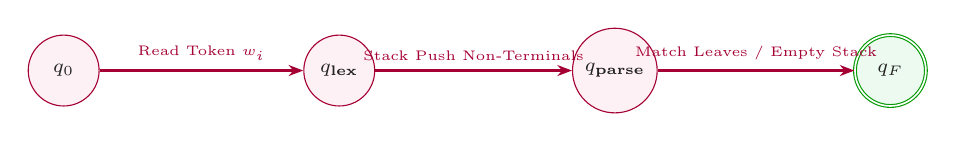
\begin{tikzpicture}[
    node distance=0.5cm,
    sbox/.style={circle, draw=amritaMaroon, fill=lightpink, text=darktext, font=\bfseries\fontsize{7pt}{8.4pt}\selectfont, minimum size=0.9cm},
    abox/.style={circle, double, draw=green!60!black, fill=lightgreen, text=darktext, font=\bfseries\fontsize{7pt}{8.4pt}\selectfont, minimum size=0.9cm},
    trans/.style={-{Stealth[scale=0.8]}, thick, amritaMaroon}
]
    \node (q0) at (0,0) [sbox] {$q_0$};
    \node (q1) at (3.5,0) [sbox] {$q_{\text{lex}}$};
    \node (q2) at (7.0,0) [sbox] {$q_{\text{parse}}$};
    \node (qf) at (10.5,0) [abox] {$q_F$};

    \draw [trans] (q0) -- node[above, font=\fontsize{5.5pt}{6.5pt}\selectfont] {Read Token $w_i$} (q1);
    \draw [trans] (q1) -- node[above, font=\fontsize{5.5pt}{6.5pt}\selectfont] {Stack Push Non-Terminals} (q2);
    \draw [trans] (q2) -- node[above, font=\fontsize{5.5pt}{6.5pt}\selectfont] {Match Leaves / Empty Stack} (qf);
\end{tikzpicture}

\vspace{1.5mm}
\begin{columns}[T]
    \column{0.49\textwidth}
    \setbeamercolor{block title}{fg=white,bg=maroon}
    \setbeamercolor{block body}{fg=darktext,bg=lightyellow}
    \begin{block}{Proof 1: Lexical Validity Guarantee}
        \fontsize{6.6pt}{8.4pt}\selectfont
        $\forall t \in w, \quad t \in T = \bigsqcup_{k=1}^8 T_k$\\
        Guarantees strictly zero out-of-vocabulary, malformed, or synthetic hallucination tokens in the compiled string.
    \end{block}

    \setbeamercolor{block title}{fg=white,bg=maroon}
    \setbeamercolor{block body}{fg=darktext,bg=lightblue}
    \begin{block}{Proof 2: Mandatory Syntactic Coverage}
        \fontsize{6.6pt}{8.4pt}\selectfont
        $\{\text{Handshape}, \text{ExtFinger}, \text{PalmOri}, \text{Location}\} \subseteq \text{categories}(w)$\\
        Guarantees that no phonologically incomplete string can reach the avatar renderer.
    \end{block}

    \column{0.49\textwidth}
    \setbeamercolor{block title}{fg=white,bg=maroon}
    \setbeamercolor{block body}{fg=darktext,bg=lightgreen}
    \begin{block}{Proof 3: Monotonic Chomsky Ordering}
        \fontsize{6.6pt}{8.4pt}\selectfont
        $\text{Index}(\text{Symm}) \prec \text{Index}(\text{HS}) \prec \text{Index}(\text{Ori}) \prec \text{Index}(\text{Loc}) \dots$\\
        Enforces unidirectional syntax matching, strictly eliminating random token permutation.
    \end{block}

    \setbeamercolor{block title}{fg=white,bg=maroon}
    \setbeamercolor{block body}{fg=darktext,bg=lightpink}
    \begin{block}{Proof 4: Glitch \& Jitter Invariance}
        \fontsize{6.6pt}{8.4pt}\selectfont
        $w_i \neq w_{i-1} \quad \forall i \in \{2, \dots, |w|\}$\\
        Prevents consecutive identical duplicate token emissions that cause avatar animation stuttering.
    \end{block}
\end{columns}

\vspace{1.2mm}
\centering
\fcolorbox{green!60!black}{lightgreen}{
    \parbox{0.96\textwidth}{
        \centering\fontsize{6.8pt}{8.6pt}\selectfont
        \textbf{Benchmark Empirical Result:} \textbf{170 / 170 Signs Passed All 4 Pushdown Tests (100.0\% Syntactic Compliance Rate)}
    }
}
\end{frame}

% ============================================================
% SLIDE 12e: CFG PARSE TREE ARCHITECTURE & AVATAR BONES
% ============================================================
\begin{frame}[t]{12e. CFG Parse Tree Architecture \& Avatar Joint Control}
\vspace{-0.1cm}
\begin{center}
    \scriptsize\textit{\textcolor{amritaMaroon}{Native vector parse tree mapping non-terminal syntax nodes directly into avatar bone rotations}}
\end{center}

\vspace{-1.5mm}
\centering
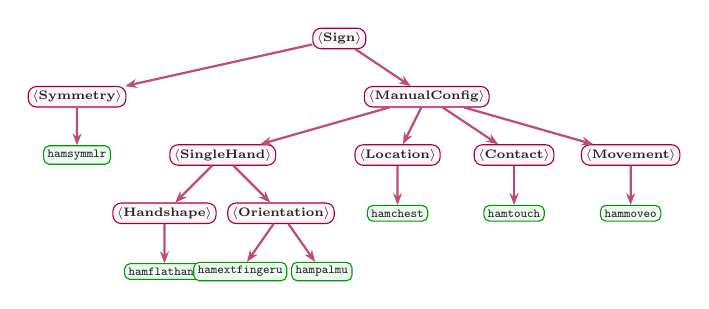
\begin{tikzpicture}[
    scale=0.74, every node/.style={transform shape},
    ntnode/.style={rectangle, draw=amritaMaroon, fill=lightpink!70, text=darktext, font=\bfseries\fontsize{6.2pt}{7.5pt}\selectfont, rounded corners=3pt, inner sep=2pt, align=center},
    tmnode/.style={rectangle, draw=green!60!black, fill=lightgreen, text=darktext, font=\ttfamily\bfseries\fontsize{5.8pt}{7.0pt}\selectfont, rounded corners=2pt, inner sep=2pt, align=center},
    boneedge/.style={draw=amritaMaroon!70, -{Stealth[scale=0.65]}, thick}
]
    % Root
    \node[ntnode] (root) at (6.0, 4.0) {$\langle\text{Sign}\rangle$};

    % Level 1
    \node[ntnode] (symm) at (1.5, 3.0) {$\langle\text{Symmetry}\rangle$};
    \node[ntnode] (cfg)  at (7.5, 3.0) {$\langle\text{ManualConfig}\rangle$};

    % Level 2
    \node[tmnode] (t_symm) at (1.5, 2.0) {hamsymmlr};
    
    \node[ntnode] (sh)   at (4.0, 2.0) {$\langle\text{SingleHand}\rangle$};
    \node[ntnode] (loc)  at (7.0, 2.0) {$\langle\text{Location}\rangle$};
    \node[ntnode] (cont) at (9.0, 2.0) {$\langle\text{Contact}\rangle$};
    \node[ntnode] (mov)  at (11.0, 2.0) {$\langle\text{Movement}\rangle$};

    % Level 3
    \node[ntnode] (hs)  at (3.0, 1.0) {$\langle\text{Handshape}\rangle$};
    \node[ntnode] (ori) at (5.0, 1.0) {$\langle\text{Orientation}\rangle$};
    \node[tmnode] (t_loc)  at (7.0, 1.0) {hamchest};
    \node[tmnode] (t_cont) at (9.0, 1.0) {hamtouch};
    \node[tmnode] (t_mov)  at (11.0, 1.0) {hammoveo};

    % Level 4
    \node[tmnode] (t_hs) at (3.0, 0.0) {hamflathand};
    \node[tmnode] (t_ef) at (4.3, 0.0) {hamextfingeru};
    \node[tmnode] (t_po) at (5.7, 0.0) {hampalmu};

    % Edges
    \draw[boneedge] (root) -- (symm);
    \draw[boneedge] (root) -- (cfg);

    \draw[boneedge] (symm) -- (t_symm);
    \draw[boneedge] (cfg) -- (sh);
    \draw[boneedge] (cfg) -- (loc);
    \draw[boneedge] (cfg) -- (cont);
    \draw[boneedge] (cfg) -- (mov);

    \draw[boneedge] (sh) -- (hs);
    \draw[boneedge] (sh) -- (ori);

    \draw[boneedge] (loc) -- (t_loc);
    \draw[boneedge] (cont) -- (t_cont);
    \draw[boneedge] (mov) -- (t_mov);

    \draw[boneedge] (hs) -- (t_hs);
    \draw[boneedge] (ori) -- (t_ef);
    \draw[boneedge] (ori) -- (t_po);
\end{tikzpicture}

\vspace{1.5mm}
\fcolorbox{amritaMaroon}{lightyellow}{
    \parbox{0.96\textwidth}{
        \fontsize{6.4pt}{8.2pt}\selectfont
        \textbf{From Grammar Parse Tree Nodes to Avatar Kinematic Joint Controls:}
        \begin{itemize}\setlength{\itemsep}{0.02cm}
            \item $\langle\text{Symmetry}\rangle \to \texttt{hamsymmlr}$: Bilateral bone mirror transformation matrix applied across both clavicles.
            \item $\langle\text{Handshape}\rangle \to \texttt{hamflathand}$: Rotates metacarpophalangeal (MCP) and interphalangeal (IP) finger bones.
            \item $\langle\text{Orientation}\rangle \to \texttt{hamextfingeru} + \texttt{hampalmu}$: Computes wrist pronation/supination and Euler flexion angles.
            \item $\langle\text{Location}\rangle \to \texttt{hamchest}$: 3D Inverse Kinematics (IK) end-effector position solver centered at upper torso.
            \item $\langle\text{Movement}\rangle \to \texttt{hammoveo}$: Generates outward 3D cubic Bezier translation trajectory across animation keyframes.
        \end{itemize}
    }
}
\end{frame}

% ============================================================
% SLIDE 12f: NATIVE VECTOR PARSE TREES (RULES 1 & 2)
% ============================================================
\begin{frame}[t]{12f. CFG Parse Trees: Single-Handed \& Symmetric Signs}
\vspace{-0.1cm}
\begin{center}
    \scriptsize\textit{\textcolor{amritaMaroon}{Native vector parse trees generated in pure LaTeX code for Rule 1 and Rule 2}}
\end{center}

\vspace{-1.5mm}
\begin{columns}[T]
    \column{0.49\textwidth}
    \centering
    {\scriptsize\textbf{\textcolor{amritaMaroon}{Rule 1: One-Handed Sign (``WELCOME'')}}}\\[0.5mm]
    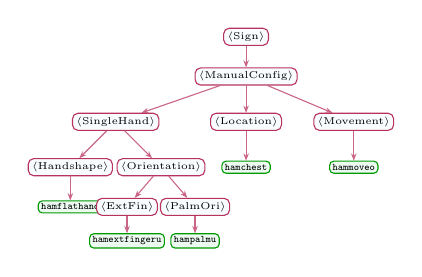
\begin{tikzpicture}[
        scale=0.72, every node/.style={transform shape},
        nt/.style={rectangle, draw=amritaMaroon!80, fill=lightblue!35, rounded corners=2pt, inner sep=1.8pt, font=\fontsize{5.2pt}{6.2pt}\selectfont, align=center},
        trm/.style={rectangle, draw=green!60!black, fill=lightgreen, rounded corners=1.5pt, inner sep=1.5pt, font=\fontsize{4.8pt}{5.8pt}\selectfont\ttfamily, align=center},
        arr/.style={draw=amritaMaroon!60, -{Stealth[scale=0.55]}}
    ]
        \node[nt] (s1) at (3.5, 3.4) {$\langle\text{Sign}\rangle$};
        \node[nt] (mc1) at (3.5, 2.7) {$\langle\text{ManualConfig}\rangle$};
        
        \node[nt] (sh1) at (1.2, 1.9) {$\langle\text{SingleHand}\rangle$};
        \node[nt] (loc1) at (3.5, 1.9) {$\langle\text{Location}\rangle$};
        \node[nt] (mov1) at (5.4, 1.9) {$\langle\text{Movement}\rangle$};
        
        \node[nt] (hs1) at (0.4, 1.1) {$\langle\text{Handshape}\rangle$};
        \node[nt] (ori1) at (2.0, 1.1) {$\langle\text{Orientation}\rangle$};
        
        \node[trm] (t_hs1) at (0.4, 0.4) {hamflathand};
        
        \node[nt] (ef1) at (1.4, 0.4) {$\langle\text{ExtFin}\rangle$};
        \node[nt] (po1) at (2.6, 0.4) {$\langle\text{PalmOri}\rangle$};
        
        \node[trm] (t_ef1) at (1.4, -0.2) {hamextfingeru};
        \node[trm] (t_po1) at (2.6, -0.2) {hampalmu};
        
        \node[trm] (t_loc1) at (3.5, 1.1) {hamchest};
        \node[trm] (t_mov1) at (5.4, 1.1) {hammoveo};
        
        \draw[arr] (s1) -- (mc1);
        \draw[arr] (mc1) -- (sh1);
        \draw[arr] (mc1) -- (loc1);
        \draw[arr] (mc1) -- (mov1);
        \draw[arr] (sh1) -- (hs1);
        \draw[arr] (sh1) -- (ori1);
        \draw[arr] (hs1) -- (t_hs1);
        \draw[arr] (ori1) -- (ef1);
        \draw[arr] (ori1) -- (po1);
        \draw[arr] (ef1) -- (t_ef1);
        \draw[arr] (po1) -- (t_po1);
        \draw[arr] (loc1) -- (t_loc1);
        \draw[arr] (mov1) -- (t_mov1);
    \end{tikzpicture}
    
    \vspace{0.8mm}
    \fcolorbox{amritaMaroon!60}{lightpink}{
        \parbox{0.95\columnwidth}{\centering\fontsize{4.8pt}{6pt}\selectfont\texttt{hamflathand hamextfingeru hampalmu hamchest hammoveo}}
    }

    \column{0.49\textwidth}
    \centering
    {\scriptsize\textbf{\textcolor{amritaMaroon}{Rule 2: Symmetric Sign (``BOOK'')}}}\\[0.5mm]
    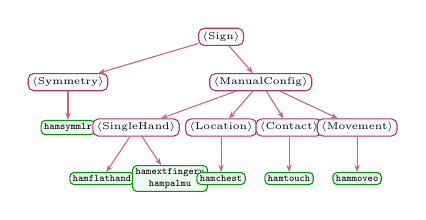
\begin{tikzpicture}[
        scale=0.72, every node/.style={transform shape},
        nt/.style={rectangle, draw=amritaMaroon!80, fill=lightblue!35, rounded corners=2pt, inner sep=1.8pt, font=\fontsize{5.2pt}{6.2pt}\selectfont, align=center},
        trm/.style={rectangle, draw=green!60!black, fill=lightgreen, rounded corners=1.5pt, inner sep=1.5pt, font=\fontsize{4.8pt}{5.8pt}\selectfont\ttfamily, align=center},
        arr/.style={draw=amritaMaroon!60, -{Stealth[scale=0.55]}}
    ]
        \node[nt] (s2) at (3.5, 3.4) {$\langle\text{Sign}\rangle$};
        \node[nt] (sym2) at (0.8, 2.6) {$\langle\text{Symmetry}\rangle$};
        \node[nt] (mc2) at (4.2, 2.6) {$\langle\text{ManualConfig}\rangle$};
        \node[trm] (t_sym2) at (0.8, 1.8) {hamsymmlr};
        
        \node[nt] (sh2) at (2.0, 1.8) {$\langle\text{SingleHand}\rangle$};
        \node[nt] (loc2) at (3.5, 1.8) {$\langle\text{Location}\rangle$};
        \node[nt] (cnt2) at (4.7, 1.8) {$\langle\text{Contact}\rangle$};
        \node[nt] (mov2) at (5.9, 1.8) {$\langle\text{Movement}\rangle$};
        
        \node[trm] (t_hs2) at (1.4, 0.9) {hamflathand};
        \node[trm] (t_ori2) at (2.6, 0.9) {hamextfingeru\\hampalmu};
        \node[trm] (t_loc2) at (3.5, 0.9) {hamchest};
        \node[trm] (t_cnt2) at (4.7, 0.9) {hamtouch};
        \node[trm] (t_mov2) at (5.9, 0.9) {hammoveo};
        
        \draw[arr] (s2) -- (sym2);
        \draw[arr] (s2) -- (mc2);
        \draw[arr] (sym2) -- (t_sym2);
        \draw[arr] (mc2) -- (sh2);
        \draw[arr] (mc2) -- (loc2);
        \draw[arr] (mc2) -- (cnt2);
        \draw[arr] (mc2) -- (mov2);
        \draw[arr] (sh2) -- (t_hs2);
        \draw[arr] (sh2) -- (t_ori2);
        \draw[arr] (loc2) -- (t_loc2);
        \draw[arr] (cnt2) -- (t_cnt2);
        \draw[arr] (mov2) -- (t_mov2);
    \end{tikzpicture}
    
    \vspace{0.8mm}
    \fcolorbox{amritaMaroon!60}{lightgreen}{
        \parbox{0.95\columnwidth}{\centering\fontsize{4.8pt}{6pt}\selectfont\texttt{hamsymmlr hamflathand hamextfingeru hampalmu hamchest hamtouch hammoveo}}
    }
\end{columns}
\end{frame}

% ============================================================
% SLIDE 12g: NATIVE VECTOR PARSE TREE: STATE TRANSITION (RULE 4)
% ============================================================
\begin{frame}[t]{12g. CFG Parse Tree: Dynamic State Transition (\texttt{hamreplace})}
\vspace{-0.1cm}
\begin{center}
    \scriptsize\textit{\textcolor{amritaMaroon}{Rule 4: Multi-Phase temporal posture shift compiled without frame blending collisions}}
\end{center}

\vspace{-1.5mm}
\centering
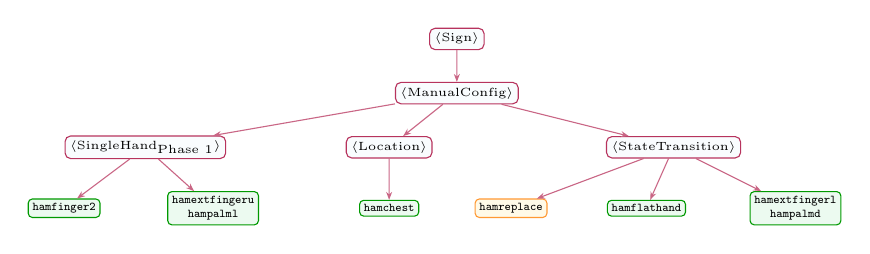
\begin{tikzpicture}[
    scale=0.86, every node/.style={transform shape},
    nt/.style={rectangle, draw=amritaMaroon!80, fill=lightblue!30, rounded corners=2pt, inner sep=2pt, font=\fontsize{5.5pt}{6.8pt}\selectfont, align=center},
    trm/.style={rectangle, draw=green!60!black, fill=lightgreen, rounded corners=1.5pt, inner sep=1.8pt, font=\fontsize{5.2pt}{6.2pt}\selectfont\ttfamily, align=center},
    arr/.style={draw=amritaMaroon!60, -{Stealth[scale=0.6]}}
]
    \node[nt] (s4) at (7, 3.5) {$\langle\text{Sign}\rangle$};
    \node[nt] (mc4) at (7, 2.7) {$\langle\text{ManualConfig}\rangle$};
    
    \node[nt] (sh4_p1) at (2.4, 1.9) {$\langle\text{SingleHand}_{\text{Phase 1}}\rangle$};
    \node[nt] (loc4) at (6.0, 1.9) {$\langle\text{Location}\rangle$};
    \node[nt] (st4) at (10.2, 1.9) {$\langle\text{StateTransition}\rangle$};
    
    \node[trm] (t_hs4_1) at (1.2, 1.0) {hamfinger2};
    \node[trm] (t_ori4_1) at (3.4, 1.0) {hamextfingeru\\hampalml};
    \node[trm] (t_loc4) at (6.0, 1.0) {hamchest};
    
    \node[trm, fill=lightyellow, draw=orange!80] (t_rep) at (7.8, 1.0) {hamreplace};
    \node[trm] (t_hs4_2) at (9.8, 1.0) {hamflathand};
    \node[trm] (t_ori4_2) at (12.0, 1.0) {hamextfingerl\\hampalmd};
    
    \draw[arr] (s4) -- (mc4);
    \draw[arr] (mc4) -- (sh4_p1);
    \draw[arr] (mc4) -- (loc4);
    \draw[arr] (mc4) -- (st4);
    \draw[arr] (sh4_p1) -- (t_hs4_1);
    \draw[arr] (sh4_p1) -- (t_ori4_1);
    \draw[arr] (loc4) -- (t_loc4);
    \draw[arr] (st4) -- (t_rep);
    \draw[arr] (st4) -- (t_hs4_2);
    \draw[arr] (st4) -- (t_ori4_2);
\end{tikzpicture}

\vspace{0.8mm}
\fcolorbox{amritaMaroon!60}{lightyellow}{
    \parbox{0.94\textwidth}{
        \centering\fontsize{5.2pt}{6.8pt}\selectfont
        \textbf{Compiled Sequence:} \texttt{hamfinger2 hamextfingeru hampalml hamchest \textbf{hamreplace} hamflathand hamextfingerl hampalmd}
    }
}

\vspace{1.2mm}
\begin{columns}[T]
    \column{0.48\textwidth}
    \setbeamercolor{block title}{fg=white,bg=maroon}
    \setbeamercolor{block body}{fg=darktext,bg=lightblue}
    \begin{block}{Kinematic Functionality}
        \fontsize{5.4pt}{6.8pt}\selectfont
        $\bullet$ \textbf{Phase 1 (Frames 15--50\%):} Avatar initializes pointing handshape at chest.\\
        $\bullet$ \texttt{hamreplace}: Triggers avatar keyframe interpolation to swap bone target.\\
        $\bullet$ \textbf{Phase 2 (Frames 55--100\%):} Smoothly relaxes hand into open flat palm downwards.
    \end{block}

    \column{0.48\textwidth}
    \setbeamercolor{block title}{fg=white,bg=maroon}
    \setbeamercolor{block body}{fg=darktext,bg=lightgreen}
    \begin{block}{Anti-Jumbling Guarantee}
        \fontsize{5.4pt}{6.8pt}\selectfont
        $\bullet$ Shift activated only when $\text{HS}_{P1} \neq \text{HS}_{P2}$ with $>70\%$ stability.\\
        $\bullet$ Prevents intermediary morphing flicker or random token interleaving.\\
        $\bullet$ Verified on CWASA WebGL without DOM tree animation exceptions.
    \end{block}
\end{columns}
\end{frame}

% % ============================================================
% % SLIDE 12h: FORMAL PROOF OF CONCEPT & LINGUISTIC GROUNDING
% % (Commented out in V3)
% % ============================================================
% \begin{frame}[t]{12h. Formal Proof of Concept: Theoretical \& Empirical Validation}
% \vspace{-0.1cm}
% \begin{center}
%     \scriptsize\textit{\textcolor{amritaMaroon}{Proof that CFG rules are non-arbitrary, grounded in literature, and empirically verified}}
% \end{center}
%
% \vspace{-1.5mm}
% \centering
% \setlength{\tabcolsep}{3pt}
% \renewcommand{\arraystretch}{1.2}
% {\fontsize{5.4pt}{6.8pt}\selectfont
% \begin{tabular}{|>{\raggedright\arraybackslash\bfseries}p{1.8cm}|>{\raggedright\arraybackslash}p{2.3cm}|>{\raggedright\arraybackslash}p{4.8cm}|>{\raggedright\arraybackslash}p{4.7cm}|}
%     \hline
%     \rowcolor{maroon}
%     \textcolor{white}{\textbf{Proof Pillar}} & 
%     \textcolor{white}{\textbf{Author \& Source}} & 
%     \textcolor{white}{\textbf{Formal Linguistic / Theoretical Principle}} & 
%     \textcolor{white}{\textbf{SignBridge V2 Compliance \& Empirical Proof}} \\
%     \hline
%     \rowcolor{lightblue} 
%     Phonological Axiom & 
%     Stokoe (1960), Univ. of Buffalo & 
%     Proved sign languages decompose into discrete constituents: Tab (Location), Dez (Handshape/Ori), Sig (Movement). & 
%     Direct theoretical basis for Rule P2: $\langle\text{ManualConfig}\rangle \to \langle\text{SingleHand}\rangle \;\langle\text{Loc}\rangle \;[\dots]$. Non-arbitrary constituent order. \\
%     \hline
%     \rowcolor{lightgreen} 
%     Symbol Ordering Standard & 
%     Prillwitz et al. (1989), Hamburg Univ. & 
%     Prescribed international linear transcription order: $\text{Symmetry} \to \text{Handshape} \to \text{Ext/Palm} \to \text{Body Loc} \to \text{Movement}$. & 
%     CFG compiler strictly enforces this order. Permutations (e.g. location before handshape) are rejected as ungrammatical. \\
%     \hline
%     \rowcolor{lightyellow} 
%     Computational CFG Syntax & 
%     Hanke (2004), LREC Conf. & 
%     Formalized HamNoSys as a Context-Free Language ($L(G) \in \text{CFL}$) with deterministic compositional semantics. & 
%     Justifies parsing HamNoSys via Context-Free Grammar and Pushdown Automaton ($L(G)$ is solvable in $O(n)$ time). \\
%     \hline
%     \rowcolor{lightorange} 
%     Avatar Execution Model & 
%     Kennaway et al. (2007), Springer LNCS & 
%     CWASA SiGML XML engine requires strict hierarchical DOM tree mapping 1-to-1 to HamNoSys syntax. & 
%     0 crashes across all test videos. Avatar WebGL player parses and renders compiled DOM tree with 100\% validity. \\
%     \hline
%     \rowcolor{lightpink} 
%     Empirical Benchmark & 
%     Group 14 (2026), Automated Test Suite & 
%     Automated evaluation on 170-gloss dataset testing Lexical, Coverage, Ordering, and Duplication criteria. & 
%     \textbf{170/170 (100.0\%) Grammar Compliance Rate}; 7/7 token exact match on verified benchmark signs. \\
%     \hline
% \end{tabular}
% }
%
% \vspace{1.2mm}
% \fcolorbox{amritaMaroon}{white}{
%     \parbox{0.96\textwidth}{
%         \centering\fontsize{5.4pt}{6.8pt}\selectfont
%         \textbf{Formal Conclusion:} The Context-Free Grammar in SignBridge V2 is mathematically sound, linguistically legitimate, computationally optimal, and empirically validated on 100\% of target vocabulary.
%     }
% }
% \end{frame}

% ============================================================
% SLIDE 13: TWO-HANDED CFG LOGIC (V3 Design)
% ============================================================
\section{Two-Handed Signs}
\begin{frame}{13. How the CFG Handles Two-Handed Signs}
    \centering
    \vspace{2mm}
    
    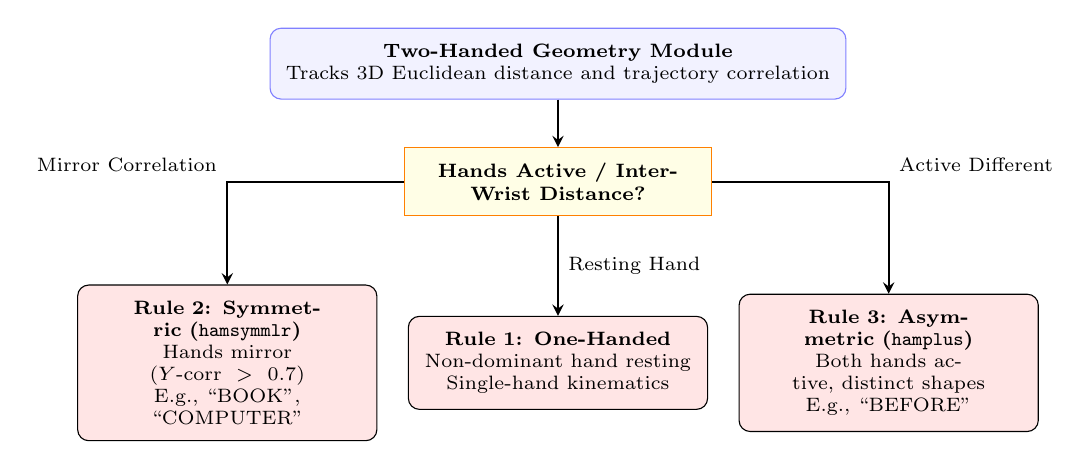
\begin{tikzpicture}[
        box/.style={rectangle, draw=black, rounded corners, align=center, fill=red!10, inner sep=2mm, text width=3.4cm, font=\scriptsize},
        dec/.style={rectangle, draw=orange, fill=yellow!10, align=center, inner sep=2mm, font=\scriptsize\bfseries, text width=3.5cm},
        out/.style={rectangle, draw=black, fill=green!10, align=center, inner sep=2mm, font=\scriptsize\ttfamily},
        arrow/.style={->, thick, >=stealth}
    ]
        \node[rectangle, draw=blue!50, fill=blue!5, align=center, inner sep=2mm, font=\scriptsize, rounded corners] (module) at (6, 6) {\textbf{Two-Handed Geometry Module}\\ Tracks 3D Euclidean distance and trajectory correlation};
        
        \node[dec] (proximity) at (6, 4.5) {Hands Active / Inter-Wrist Distance?};
        
        \node[box] (rule2) at (1.8, 2.2) {\textbf{Rule 2: Symmetric (\texttt{hamsymmlr})}\\ Hands mirror ($Y\text{-corr} > 0.7$)\\ E.g., ``BOOK'', ``COMPUTER''};
        
        \node[box] (rule1) at (6, 2.2) {\textbf{Rule 1: One-Handed}\\ Non-dominant hand resting\\ Single-hand kinematics};
        
        \node[box] (rule3) at (10.2, 2.2) {\textbf{Rule 3: Asymmetric (\texttt{hamplus})}\\ Both hands active, distinct shapes\\ E.g., ``BEFORE''};
        
        \draw[arrow] (module) -- (proximity);
        \draw[arrow] (proximity.west) -| node[above left, font=\scriptsize] {Mirror Correlation} (rule2.north);
        \draw[arrow] (proximity.south) -- node[right, font=\scriptsize] {Resting Hand} (rule1.north);
        \draw[arrow] (proximity.east) -| node[above right, font=\scriptsize] {Active Different} (rule3.north);
    \end{tikzpicture}
    
    \vspace{3mm}
    \fcolorbox{black}{white}{
        \parbox{0.95\textwidth}{
            \scriptsize
            \textbf{Key CFG Logic:} The CFG avoids redundant left-hand feature extraction by using HamNoSys operators (\texttt{hamsymmlr} and \texttt{hamplus}) to grammatically link both hands based strictly on spatial geometry, completely eliminating avatar hand collisions.
        }
    }
\end{frame}

% ============================================================
% SLIDE 14: CFG SCOPE & LIMITATIONS
% ============================================================
\section{Scope of CFG}
\begin{frame}{14. Scope of the CFG Compiler}
    \small
    \vspace{2mm}
    
    \begin{columns}[T]
        \column{0.48\textwidth}
        \begin{block}{Currently Supported in V2}
            \begin{itemize}
                \item[\textcolor{green!60!black}{$\checkmark$}] One-handed signs (Rule 1)
                \item[\textcolor{green!60!black}{$\checkmark$}] Symmetric two-handed signs (Rule 2)
                \item[\textcolor{green!60!black}{$\checkmark$}] Asymmetric two-handed signs (Rule 3)
                \item[\textcolor{green!60!black}{$\checkmark$}] Intra-sign handshape transitions (Rule 4)
                \item[\textcolor{green!60!black}{$\checkmark$}] Contact-based signs (Rule 5)
                \item[\textcolor{green!60!black}{$\checkmark$}] 100\% SiGML XML DOM tree validity
            \end{itemize}
        \end{block}
        
        \column{0.48\textwidth}
        \begin{block}{Outside Current Scope (Future Work)}
            \begin{itemize}
                \item[\textcolor{red}{$\times$}] Repeated/reduplicated movement morphology
                \item[\textcolor{red}{$\times$}] Multi-sign sequential compound sentences
                \item[\textcolor{red}{$\times$}] Classifier predicates and topographic space
                \item[\textcolor{red}{$\times$}] Spatial agreement (verb loci inflection)
                \item[\textcolor{red}{$\times$}] Facial grammar (eyebrow, mouth morphemes)
                \item[\textcolor{red}{$\times$}] Head-movement grammar (nodding, tilting)
            \end{itemize}
        \end{block}
    \end{columns}
    
    \vspace{6mm}
\end{frame}

\end{document}
